\documentclass[11pt]{article}
\usepackage[margin=1in]{geometry}
% Math packages.
\usepackage{amsmath,amssymb,amstext,amsfonts}
% Add figures.
\usepackage{graphicx}

% Metadata
\author{FCM Student}
\title{Example Solution Report for Example Assignment}

\begin{document}

\maketitle

\section{Executive Summary}

In this report, we consider the big-$O$ order of accuracy for the forward, backward, and central finite difference approximations to the derivative of a function. Analytic derivations are confirmed empirically by a method of best-fit line under logarithmic transformation of the absolute error. Results are obtained and discussed for two functions, $f_1(x) = \sin(x)$ and $f_2(x) = \exp(-0.5x^2)$.

\section{Statement of the Problem}

The numerical approximation of derivatives is important in scientific- and mathematical-computing applications, e.g., in the numerical approximations to ODEs. Finite difference methods, which often depend on some parameter, $h$, can be used for these approximations, and the accuracy and convergence properties of the approximation often depends on the value of this parameter. We analyze these properties for the forward, backward, and central difference approximations, respectively:

\begin{enumerate}
    \item $\displaystyle F_h[f](x) = \frac{f(x+h) - f(x)}{h}$
    \item $\displaystyle B_h[f](x) = \frac{f(x) - f(x-h)}{h}$
    \item $\displaystyle C_h[f](x) = \frac{f(x+h) - f(x-h)}{2h}$
\end{enumerate}

\section{Description of the Mathematics}

\subsection{Determining the Order of Accuracy}

A finite difference approximation to the true derivative at some point, $x$, is often $O(h^p)$ for some positive integer, $p$, i.e., the approximation is within $Ch^p$ to the true derivative whenever $0 < h < \delta$ for some $C$ and appropriately chosen $\delta$. We derive the value, $p$, for forward, backward, and central difference methods in this section. Throughout, we assume that the function, $f(x)$, can be expanded as necessary using Taylor's theorem.

\subsubsection{Analytic Derivation of Accuracy Order}
\label{subsection:accuracy-order-derivation}
First, 
$$
    f(t) = f(x) + f'(x)(t-x) + \frac{f''(\xi)}{2}(x-h)^2
$$
by Taylor expansion to second-order, so that
$$
    f(x+h) = f(x) + f'(x)h + \frac{f''(\xi)}{2}h^2
$$
and finally,
$$
    \frac{f(x+h)-f(x)}{h} = f'(x) + \frac{f''(\xi)}{2}h = f'(x) + O(h)
$$
Thus, $F_h[f](x)$ is $O(h)$. Similarly, evaluating the second-order expansion at $x-h$, we obtain, 
$$
    \frac{f(x)-f(x-h)}{h} = f'(x) - \frac{f''(\xi)}{2}h = f'(x) + O(h)
$$
Thus, $B_h[f](x)$ is $O(h)$. Finally, by taking Taylor expansion to third-order,
$$
    f(t) = f(x) + f'(x)(t-x) + \frac{f''(x)}{2}(t-x)^2 + \frac{f^{(3)}(\mu)}{6}(t-x)^3
$$
we then obtain,
$$
    f(x+h)-f(x-h) = 2f'(x)h  + \frac{f^{(3)}(\mu)}{3}h^3
$$
Thus, $C_h[f](x)$ is $O(h^2)$.

\subsubsection{Method for Empirical Estimation of Accuracy Order\protect\footnote{The method described in this section is equivalent to the ``normal equation" approach. Ideally, a more numerically stable method should be used to solve this linear least-squares problem, e.g., the $QR$ decomposition.}}

\label{subsection:accuracy-estimate}

In this section, we describe a method for estimating the order of the accuracy of a numerical approximation by finding the slope of the best-fit line in log-space. Suppose we use some difference method, $D_h[f](x)$, for approximating the derivative, $f'(x)$.

We consider some fixed number of $h$ values, say $h_1, h_2, \ldots, h_m$, and for each, we measure the absolute error,
$$
    a_i := |D_{h_i}[f](x)-f'(x)|
$$
Assuming $a \approx Ch^p$ for some $C$ and $p$, we have that $\log(a) \approx \log(C) + p\log(h)$. We make the transformations, $u_i = \log(h_i)$, $v_i = \log(a_i)$, and denote $b=\log(C)$. The best parameters for the line, $a = b + pu$, are determined in the least-squares sense, i.e., those that minimize:
$$
    L(b,p) := \sum_{i=1}^m \left(b+pu_i - v_i\right)^2
$$
By taking partial derivatives, and setting to zero, we obtain a linear system:
$$
    \begin{bmatrix}
        m          & \sum_i u_i \\
        \sum_i u_i & \sum_i u_i^2
    \end{bmatrix}
    \begin{bmatrix} b \\ p \end{bmatrix}
    =
    \begin{bmatrix} \sum_i v_i \\ \sum_i u_iv_i \end{bmatrix}
$$
Solving the system for $b$ and $p$, yields the parameters of the best-fit line,
$$
    \hat{b} = \frac{\left(\sum_i u_i^2\right) \left(\sum_i v_i\right) - \left(\sum_i u_i\right)\left(\sum_i u_iv_i\right)}{m\sum_i u_i^2 - \left(\sum_i u_i \right)^2}
$$
and
$$
    \hat{p} = \frac{m\left(\sum_i u_iv_i\right) - \left(\sum_i u_i\right)\left(\sum_i v_i\right)}{m\sum_i u_i^2 - \left(\sum_i u_i \right)^2}
$$
Therefore, $\hat{p}$, yields an empirical estimate of the order of the accuracy of the finite difference approximation to the derivative.

\section{Description of the Algorithms and Implementation}

The finite difference methods each are translated directly into respective functions in \texttt{C++}, which accept three arguments: (1) a function, $f$, (2) a value, $x$, and (3) a value, $h$. For example, if a function, \texttt{func}, is previously defined, then \texttt{fdiff::forward(func, 1.2, 1e-3)} returns the forward difference approximation to the derivative of \texttt{func} at $x=1.2$ with $h=10^{-3}$.

\section{Description of the Experimental Design and Results}

For each finite difference method, function, and $x$-value, the order of the accuracy is first estimated by plotting, in logscale, the obtained absolute error against increasing values of $h$, and visually estimate the slope of the resulting line. We also quantify the slope, employing the method described in Section~\ref{subsection:accuracy-estimate}. Specifically, we choose $h_i = 10^{-1-6(i-1)/(m-1)}$, $i=1,\ldots, m$. This yields $m$ values of $h$ that are equally spaced after a $\log_{10}$ transformation, such that $h_1 = 10^{-1}$ and $h_m = 10^{-7}$. We choose $m=25$.

In Figures~\ref{fig:func1-results}~and~\ref{fig:func2-results}, the absolute error for both required functions, $f_1$ and $f_2$, and the required values of $x$, is plotted against increasing values of $h$. For both functions, we visually estimate in Figures~\ref{fig:func1-results}~and~\ref{fig:func2-results} that the forward and backward difference methods yield a slope of approximately 1. We observe, however, that for the central difference method, for both functions and for values of $h$ less than approximately $10^{-5}$ that the absolute error begins to increase and behave more erratically due to floating-point rounding error.

In Tables~\ref{tab:order-estimates-f1}~and~\ref{tab:order-estimates-f2}, the visually estimated slopes match the estimated values from the method of Section~\ref{subsection:accuracy-estimate}. We find values of approximately 1 (the expected analytic slope) for the forward and backward difference methods for both functions, $f_1$ and $f_2$, and each $x$-value tested, which agrees with the analytic order derived. We find that the estimated order of accuracy for the central difference method is skewed away from $2$ (the expected analytic slope for this method) when values of $h$ below $10^{-5}$. We observe (also in Tables~\ref{tab:order-estimates-f1}~and~\ref{tab:order-estimates-f2}) that by excluding these cases where numerical round-off becomes an issue, that we obtain order of accuracy estimates that agree with the analytically derived order of accuracy for the central difference method.

\section{Conclusions}

Our results illustrate the big-$O$ accuracy of the forward, backward, and central finite difference approximations to the derivative of a function. We found that numerical rounding-error affected the accuracy of the  central difference approximation for values of $h$ below $10^{-5}$. We suspect that similar findings would be obtained for the forward and backward difference methods as well, for smaller values of $h$ than those discussed in this report. This raises the question of how the value of $h$ should be chosen for a given function and finite difference method. Ideally, $h$ would be chosen in such manner so that the difference approximation maintains some acceptable level of error against the true derivative for all desired values of $x$. Another topic not considered in this report is how boundaries should be handled. In some circumstances, it may not be possible to sample a function beyond some point (or set of points), thus rendering some finite difference unsuitable for certain points. Is it possible, for example, to use the higher-order, central difference method in interior regions, and switch to some other second-order finite difference method not discussed here on the boundaries? Answers to such questions and related ones could be studied further in the future or found perhaps in the literature.

\section{Tables and Figures}

\begin{figure}[!ht]
    \centering
    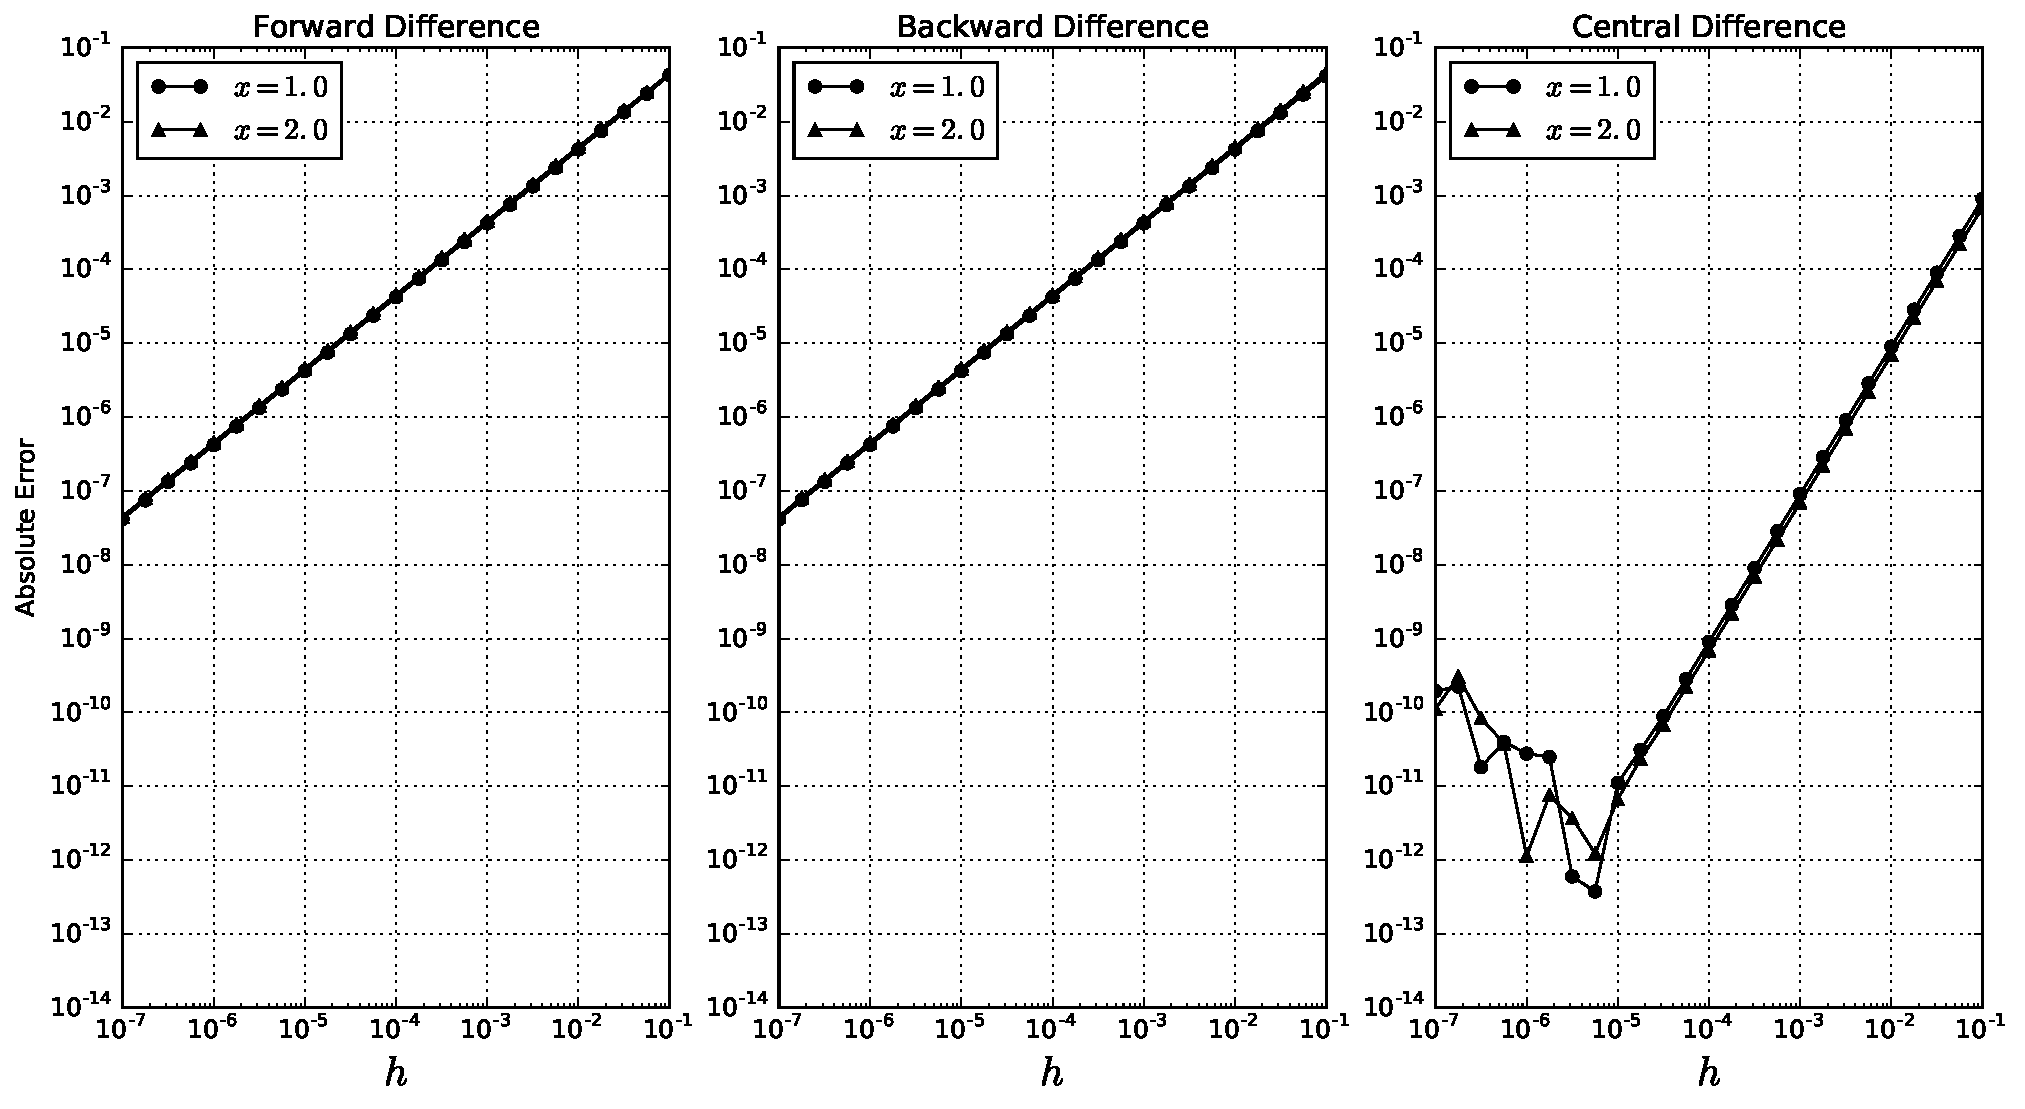
\includegraphics[width=\textwidth]{../figures/f1.pdf}
    \caption{Error results for $f_1(x) = \sin(x)$ for the three difference methods, shown in log scale.}
    \label{fig:func1-results}
\end{figure}

\begin{figure}[!hb]
    \centering
    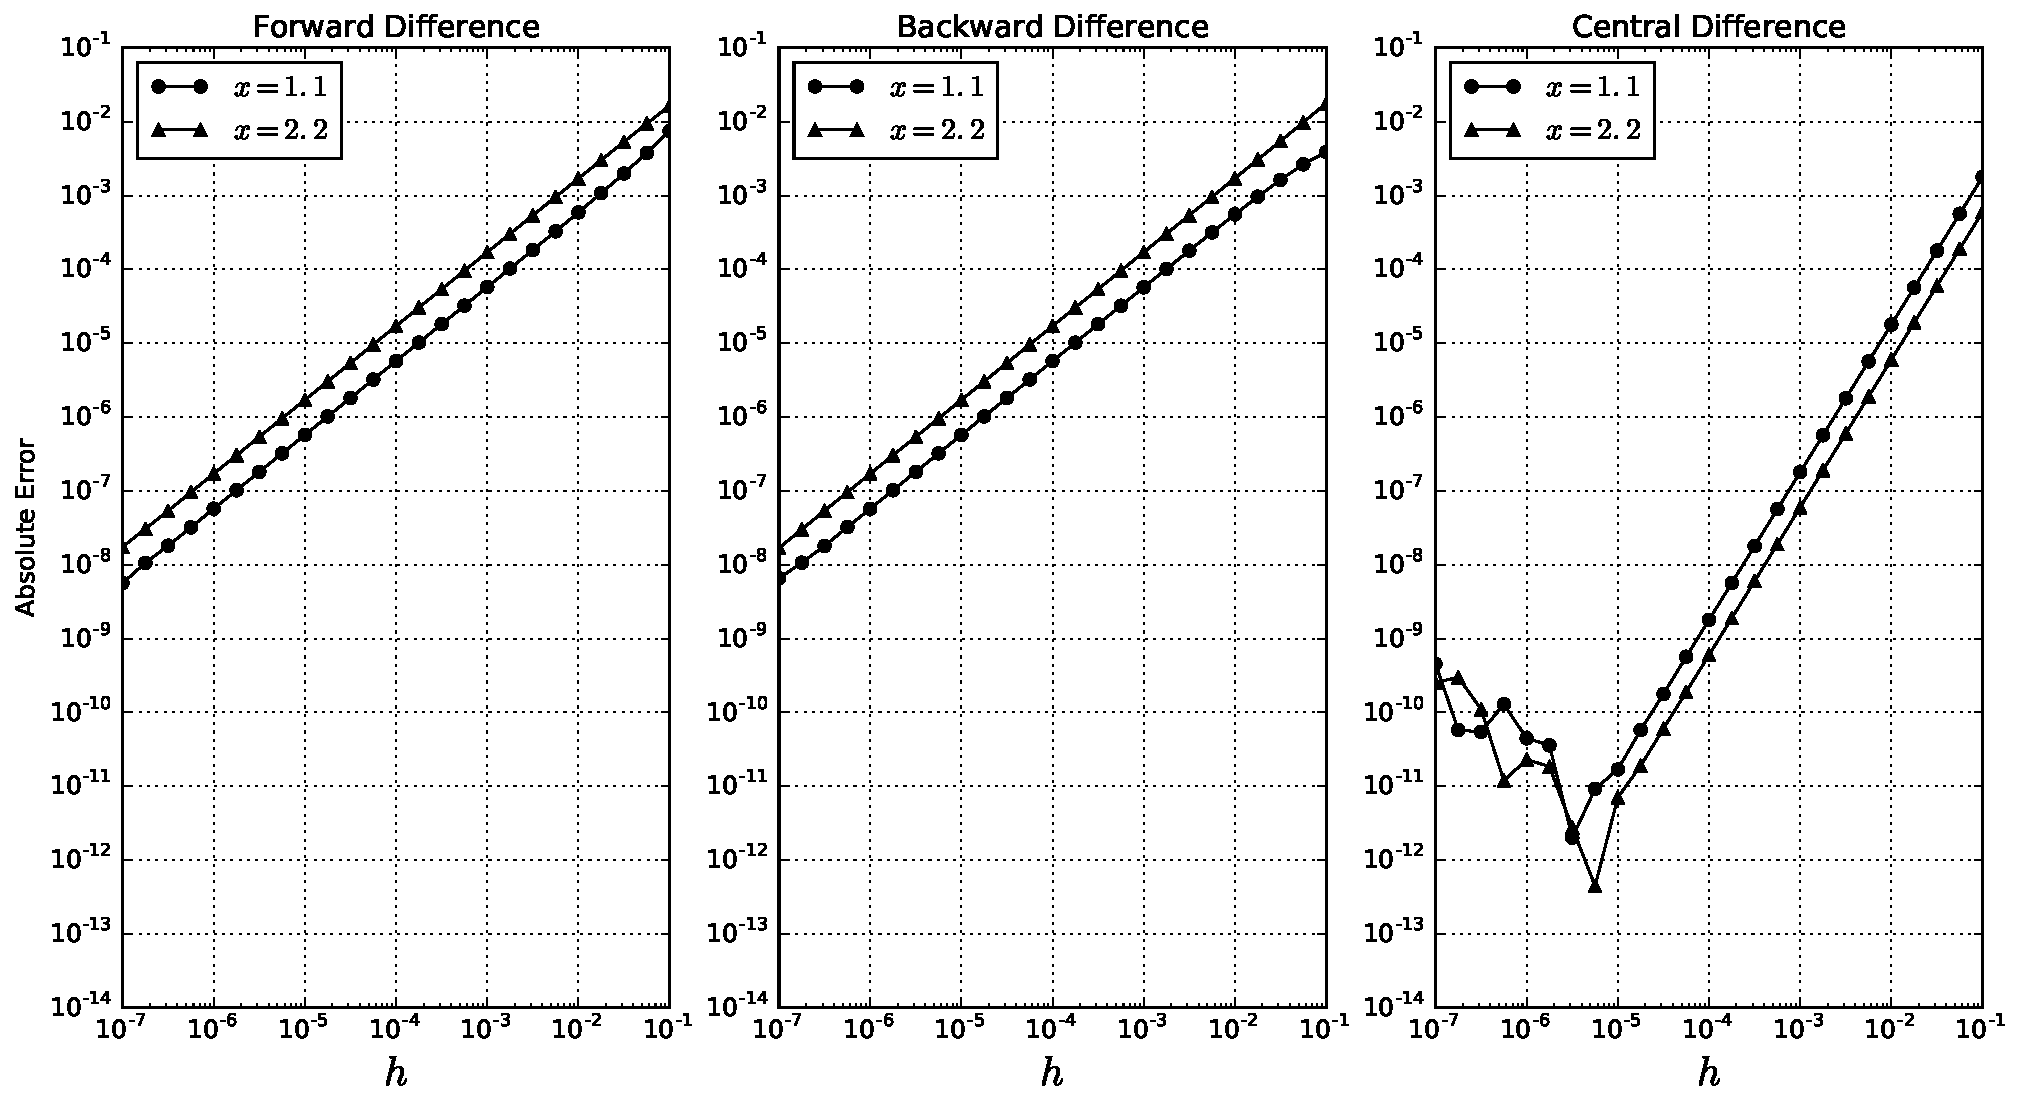
\includegraphics[width=\textwidth]{../figures/f2.pdf}
    \caption{Error results for $f_2(x) = \exp(-0.5x^2)$ for the three difference methods, shown in log scale.}
    \label{fig:func2-results}
\end{figure}

\begin{table}[!ht]
    \centering
    \begin{tabular}{|c|c|c|c|c|}
        \hline
                & Forward & Backward & Central & Central ($< 10^{-5}$ excluded) \\
        \hline
        $x=1.0$ & 1.0008  & 0.9995   & 1.3607  & 1.9944 \\
        \hline
        $x=2.0$ & 0.9997  & 1.0006   & 1.3454  & 2.0067 \\
        \hline
    \end{tabular}
    \caption{Order of accuracy estimates ($\hat{p}$) by method of Section~\ref{subsection:accuracy-estimate} for $f_1(x) = \sin(x)$.}
    \label{tab:order-estimates-f1}

    \vspace{0.5in}

    \begin{tabular}{|c|c|c|c|c|}
        \hline
                & Forward & Backward & Central & Central ($< 10^{-5}$ excluded) \\
        \hline
        $x=1.1$ & 1.0089 & 0.9853   & 1.3629  & 2.0021  \\
        \hline
        $x=2.1$ & 0.9984 & 1.0014   & 1.2977  & 1.9916  \\
        \hline
    \end{tabular}
    \caption{Order of accuracy estimates ($\hat{p}$) by method of Section~\ref{subsection:accuracy-estimate} for $f_2(x) = \exp(-0.5x^2)$.}
    \label{tab:order-estimates-f2}
\end{table}

\end{document}
